\subsection{Инфраструктура LLVM MLIR}
\label{impl:mlir} % \index{Chapter5}

Как было сказано в главе \ref{sec:Compilers}, компиляторы
решали сходные задачи, но они отличались некоторыми деталями, из-за чего
приходилось создавать новый компилятор и пересоздавать большое количество
компонентов. В связи с этим сообщество разработчиков LLVM придумали и реализовали
переиспользуемую и расширяемую инфраструктуру MLIR.

Основная концепция MLIR --- диалекты. Диалект объединяет в себе типы, операции
и их преобразования на каком-либо уровне абстракции. В MLIR существует более 40
встроенных диалектов, имплентация собственных диалектов возможна с помощью
декларативного языка \textit{ODS} или на языке C++.

Рассмотрим некоторые диалекты, которые будут использованы в данной работе.

\begin{enumerate}
    \item \textit{HLO} --- диалект, который позволяет представлять модели
          нейросетей, написанных на tensorflow, в представлении MLIR. Несмотря
          на то, что он не является стандартным и представлен в виде отдельного
          репозитория, пользуется популярностью благодаря широкой
          известности tensorflow.

    \item \textit{tensor} --- диалект для представления тензоров и операций,
          позволяющих менять форму тензоров, изменять их размеры,
          <<вырезать>> и <<вставлять>> части из них. Стоит отметить, на
          данном уровне абстракции считается, что тензоры не имеют какого-то
          конкретного расположения в памяти. Этим они похожи на виртуальные
          регистры из теории компиляторов.

    \item \textit{memref} --- диалект, который абстрагирует работу с многомерными
          массивами. Операции в этом диалекте схожи с операциями из диалекта
          tensor, но этих диалектов есть существенное отличие: memref является
          представлением реальных объектов.

    \item \textit{affine} --- диалект, который предоставляет возможность работы с
          аффинными циклами и преобразованиями над ними, тем самым реализуя
          возможности для полиэдральной компиляции.

    \item \textit{scf} (\textit{structured control flow}) --- диалект, в котором
          представлен структурный поток исполнения (т.е. в виде системы вложенных
          блоков).

    \item \textit{cf} (\textit{control flow}) --- диалект, предсталяющий
          исполнение в виде графа потока управления.

    \item \textit{func} --- диалект, реализующий концепцию функций, их вызова,
          передачи аргументов, возвращения значения.

    \item \textit{transform} --- диалект, необходимый для реализации
          преобразований внутри одного диалекта. С его помощью операция
          предсталяется в виде одной или нескольких операций (зачастую, более
          эффективных по производительности, чем исходная), что позволяет
          подготовить код для дальнейшего lowering-а или оптимизировать его.

    \item \textit{llvm} --- самый низкоуровневый диалект, реализующий семантику
          LLVM IR. Его можно перевести в LLVM IR непосредственно, после чего
          воспользоваться другими средствами LLVM для компиляции. Отметим, что
          получение кода именно в таком представлении является нашей
          непосредственной задачей.

    \item \textit{bultin} --- базовый диалект, предоставляющий базовые типы
          данных и некоторые служебные объекты (например, аттрибуты).

    \item \textit{arith} --- диалект операций над элементарными типами.
\end{enumerate}

Выше были перечислены лишь те диалекты, которые непосредственно будут
использованы во время lowering-а из HLO в llvm. Помимо в них в MLIR существует
большое количество других диалектов, например, для графических ускорителей (GPU),
для векторных инструкций (AVX512), для распараллеливания исполнения программ
(OpenMP) и другие. Общая диаграмма диалектов и их соотношения представлена на
рисунке ниже.

\begin{figure}[h!]
    \centering
    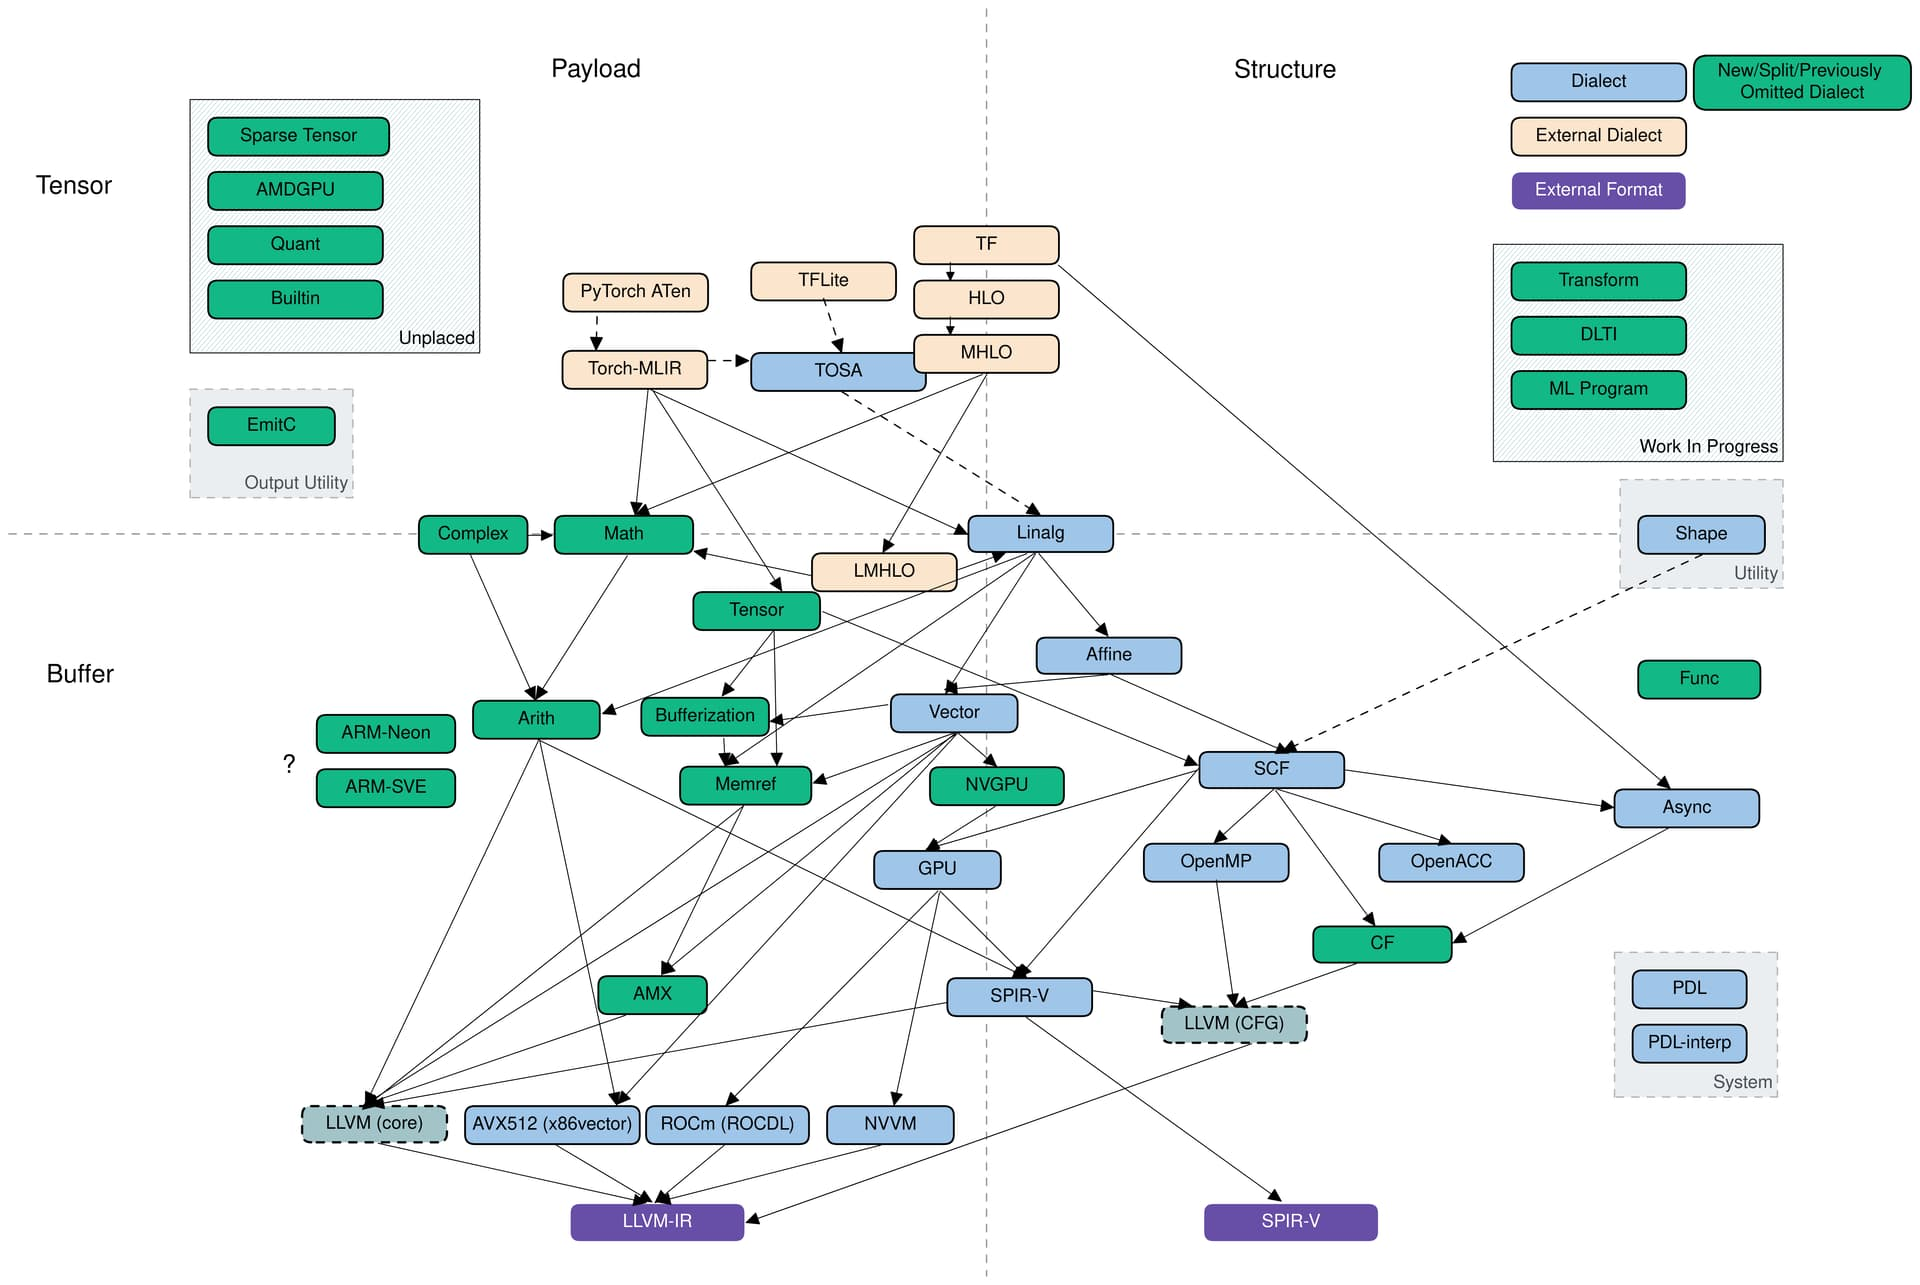
\includegraphics[scale=0.25]{MLIR_Dialects.jpg}
    \caption{Структура проекта MLIR и соотношения диалектов в них}
\end{figure}
